\bigskip 
\bigskip 
\subsubsection{Contenido}
\bigskip 
%\begin{wrapfigure}{r}{0.5\textwidth}
%  \begin{center}
%    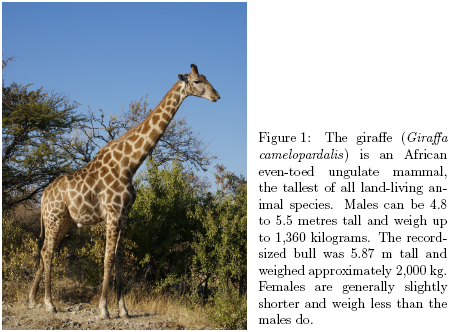
\includegraphics[width=0.48\textwidth]{./ingles/Latex_example_sidecap.jpg}
%  \end{center}
%\end{wrapfigure}

\begin{description}
\item[Nombre:] Negroni
\item[Cristaleria:] Rock glass (6oz / 180cc)
\item[M\'etodo de elaboraci\'on:] Batido
\item[Decoraci\'on:] C\'ascara de naranja
\end{description}

\begin{table}[h]
\caption{Ingredientes y proporciones} 
\label{tab:fonts}
\begin{center}       
\begin{tabular}{|l|l|l|c|l|} %% this creates two columns
%% |l|l| to left justify each column entry
%% |c|c| to center each column entry
%% use of \rule[]{}{} below opens up each row
\hline
\rule[-1ex]{0pt}{3.5ex}  \textbf{Producto} & \textbf{Bebida} & \textbf{Marca} & \textbf{Volumen} & \textbf{Fraccion}  \\
\hline
\rule[-1ex]{0pt}{3.5ex}  Aguardiente & Gin 			& Boodles British 		& 1 oz / 30 cc 	&  	\\
\hline
\rule[-1ex]{0pt}{3.5ex}  Licor 		& Campari	 	& 				& 1 oz / 30 cc 		&  	\\
\hline
\rule[-1ex]{0pt}{3.5ex}  Vermouth	& Cinzano Rosso 	& Cinzano 				& 1 oz / 30 cc					& 	\\
\hline
\rule[-1ex]{0pt}{3.5ex}  Fruta 		& Naranja		& C\'ascara		& 								& 	\\
\hline
\end{tabular}
\end{center}
\end{table} 
\bigskip 

%%-----------------------------------------------------------
\subsubsection{Formato de elaboraci\'on} 
\label{sec:title}
\bigskip 
\begin{center}
\begin{enumerate}
\item Colocar hielo en una coctelera.
\item Colocar el gin, campari y cinzano en la coctelera.
\item Tapar la coctelera y batir.
\item Servir en vaso Rock Glass.
\item Aromatizar y decorar con la c\'ascara de naranja.
\end{enumerate}
\end{center}
\bigskip 
\bigskip 
%%%%%%%%%%%%%%%%%%%%%%%%%%%%%%%%%%%%%%%%%%%%%%%%%%%%%%%%%%%%%

\subsubsection{Notas}
\bigskip 
\begin{center}
\raggedright{}Servir con sorbete.
\end{center} 

\subsubsection{Informaci\'on extra}
\bigskip
\begin{center}
\medskip 
\raggedright{ \textbf{Or\'igenes de este trago}} \\ 
\medskip

{\justifying{
\indent El Negroni, cuyo nombre refiere al apellido de su creador el Conde Camilo Negroni, se invent\'o aproximadamente en el a\~no 1920, en Florencia. El c\'octel preferido del se\~nor Negroni era el Americano, pero el cre\'ia que a\'un pod\'ia ser mejor y m\'as fuerte, por eso le pidi\'o a su cantinero que sustituyese la soda por gin, y as\'i naci\'o el Negroni, un trago espectacular. Este trago se considera como un excelente aperitivo y uno de los tragos m\'as importantes de Italia.
}\par}
\end{center}